\section{Finite Abel cancellations do not control the exponential sum}
\label{app:abel-obstruction}

Equation~\eqref{eq:prime-tail-double-zero} proves a double zero in
an Abel weight at \(s=1\). It does not prove the signed
exponential-kernel estimate \eqref{eq:prime-tail-target}. We test
the proposed implication in the larger class of bounded real
coefficients. The test below is explicit and uses neither RH
nor a hypothetical zero of the Riemann zeta function.

\begin{theorem}[A prescribed finite set of vanishing moments]
\label{thm:abel-obstruction}
Let \(k\ge1\) be an integer, \(1/2<\beta<1\), and \(\gamma>0\).
There is a real sequence \((a_n)\), with \(|a_n|\le1\), such that:
\begin{enumerate}
\item Its Dirichlet series \(D_a(s)=\sum_{n\ge1}a_nn^{-s}\)
  is absolutely convergent on \(\operatorname{Re}s>\beta\), and
  \[
   D_a^{(j)}(1)=
      \sum_{n\ge1}\frac{a_n(-\log n)^j}{n}=0
        \qquad(0\le j<k).
  \]
\item It has a meromorphic continuation with simple poles at
  \(\beta+i\gamma\) and \(\beta-i\gamma\). The Mellin transform
  \(\Gamma(s)D_a(s)\) still has those poles and has a zero of
  order at least \(k\) at \(s=1\).
\item Its exponentially smoothed sum satisfies
  \[
   S_a(X):=\sum_{n\ge1}a_ne^{-n/X}
    =\varepsilon\,\operatorname{Re}
        \bigl(\Gamma(\beta+i\gamma)X^{\beta+i\gamma}\bigr)
       +O_{k,\beta,\gamma}(1)
  \]
  for some explicitly specified \(\varepsilon>0\).
  Consequently
  \[
   \limsup_{X\to\infty}\frac{S_a(X)}{X^\beta}
       =\varepsilon|\Gamma(\beta+i\gamma)|,\qquad
   \liminf_{X\to\infty}\frac{S_a(X)}{X^\beta}
       =-\varepsilon|\Gamma(\beta+i\gamma)|.
  \]
\end{enumerate}
In particular, these \(k\) exact moment cancellations do not imply
\(S_a(X)=O(X^{1/2+\eta})\) when \(0<\eta<\beta-1/2\).
\end{theorem}

\begin{proof}
Put \(z=\beta+i\gamma\) and
\(r_n=n^{\beta-1}\cos(\gamma\log n)\). Initially retain this
coefficient except on the finite set
\[
 \mathcal S=\{2^m:0\le m<k\}.
\]
For \(0\le j<k\) define the absolutely convergent real moments
\[
 t_j=\sum_{n\notin\mathcal S}
              \frac{r_n(-\log n)^j}{n}.
\]
Convergence follows from
\(|r_n|(\log n)^j/n\le n^{\beta-2}(\log n)^j\).
We choose real numbers \(b_m\) at the indices \(2^m\) by
\begin{equation}\label{eq:moment-system}
 \sum_{m=0}^{k-1}\frac{b_m(-m\log2)^j}{2^m}
       =-t_j\qquad(0\le j<k).
\end{equation}
The matrix is invertible: after nonzero row and column
scalings it is the Vandermonde matrix \((m^j)_{j,m=0}^{k-1}\).
Its determinant is
\(\prod_{0\le m<n<k}(n-m)\ne0\).

There is also a direct finite formula for the solution. Set
\[
 \ell_m(x)=\prod_{\substack{0\le n<k\\n\ne m}}
                    \frac{x-n}{m-n}
           =\sum_{j=0}^{k-1}\ell_{m,j}x^j,\qquad
 s_j=-\frac{t_j}{(-\log2)^j}.
\]
Then
\[
 b_m=2^m\sum_{j=0}^{k-1}\ell_{m,j}s_j.
\]
Indeed, applying the moment functional
\(x^j\mapsto s_j\) to \(\ell_m\) inverts the moment system.
All the numbers \(\ell_{m,j}\) are rational.

Choose
\[
 \varepsilon=\frac1{1+\max_{0\le m<k}|b_m|}>0,\qquad
 a_n=\begin{cases}
       \varepsilon b_m,&n=2^m\in\mathcal S,\\
       \varepsilon r_n,&n\notin\mathcal S.
      \end{cases}
\]
Since \(|r_n|\le1\), all coefficients have modulus at most
one. The moment equations prove the first assertion, including
termwise differentiation at one.

For complex \(s\), absolute convergence initially gives the
holomorphic identity
\begin{equation}\label{eq:model-dirichlet}
 D_a(s)=\frac{\varepsilon}{2}
    \left(\zeta(s+1-\beta-i\gamma)
          +\zeta(s+1-\beta+i\gamma)\right)
       +\varepsilon\sum_{m=0}^{k-1}
          (b_m-r_{2^m})2^{-ms}.
\end{equation}
The finite sum is entire. The two shifted zeta functions
have distinct simple poles at the asserted points, each
with residue \(\varepsilon/2\). They are regular at one.
The moment equations give a zero there of order at least
\(k\). Multiplication by \(\Gamma(s)\), which is nonzero
and holomorphic at these points, preserves both assertions.
\footnote{For complex \(s\), the average of the two shifted
zeta functions in \eqref{eq:model-dirichlet} must be used.
Writing its real part instead would destroy holomorphy.
The displayed poles are constructed poles, not assertions
that \(\zeta(\beta\pm i\gamma)=0\).}

It remains to justify the smoothed asymptotic without any
unproved contour shift. For \(X\ge1\), apply elementary
sum--integral comparison to
\(f_X(t)=t^{z-1}e^{-t/X}\) on \([1,\infty)\). The integral
of its absolute derivative is at most
\[
 |z-1|\int_1^\infty t^{\beta-2}\dd t
   +X^{-1}\int_1^\infty t^{\beta-1}e^{-t/X}\dd t
 \le\frac{|z-1|}{1-\beta}+\Gamma(\beta).
\]
The omitted integral on \((0,1)\) has modulus at most
\(1/\beta\). Comparing on each interval \([n,n+1]\)
therefore gives the uniform estimate
\[
 \sum_{n\ge1}n^{z-1}e^{-n/X}
       =\int_0^\infty t^{z-1}e^{-t/X}\dd t+O_{\beta,\gamma}(1)
       =\Gamma(z)X^z+O_{\beta,\gamma}(1).
\]
The last identity is Euler's convergent gamma integral
\cite[\S5.9(i)]{dlmf-gamma}, here applied with
\(\operatorname{Re}z>0\). The finite coefficient changes
add only \(O_{k,\beta,\gamma}(1)\). Taking real parts
proves the asymptotic.

Finally choose
\(\log X_j=(2\pi j-\arg\Gamma(z))/\gamma\)
and the analogous sequence with an added \(\pi/\gamma\).
The two limiting normalized values have opposite signs and
the stated modulus. The uniform asymptotic bounds the
absolute normalized value by that same modulus, proving
the exact limit superior and inferior.
\end{proof}

\begin{figure}[ht]
\centering
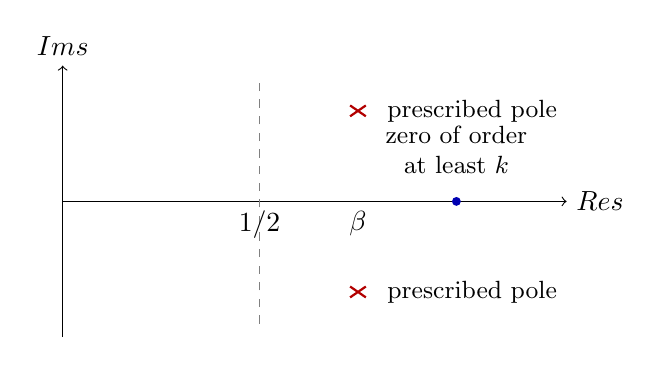
\begin{tikzpicture}[x=5cm,y=1.15cm]
 \draw[->] (0,0)--(1.28,0) node[right] {\(\operatorname{Re}s\)};
 \draw[->] (0,-1.5)--(0,1.5) node[above] {\(\operatorname{Im}s\)};
 \draw[dashed,gray] (.5,-1.35)--(.5,1.35);
 \node[below] at (.5,0) {\(1/2\)};
 \node[below] at (.75,0) {\(\beta\)};
 \fill[blue!70!black] (1,0) circle(1.6pt);
 \node[above,align=center,font=\small] at (1,.2)
     {zero of order\\at least \(k\)};
 \draw[red!70!black,thick] (.73,.94)--(.77,1.06)
                            (.73,1.06)--(.77,.94);
 \draw[red!70!black,thick] (.73,-.94)--(.77,-1.06)
                            (.73,-1.06)--(.77,-.94);
 \node[right,font=\small] at (.8,1) {prescribed pole};
 \node[right,font=\small] at (.8,-1) {prescribed pole};
\end{tikzpicture}
\caption{A model Dirichlet series in Theorem~\ref{thm:abel-obstruction}.
Any fixed number of vanishing moments at one can coexist with
the two prescribed poles. These are not claimed zeros of
the Riemann zeta function.}\label{fig:model-mellin-poles}
\end{figure}

The construction can also start with
\(r_n=n^{\beta-1}\cos(\gamma\log n-\arg\Gamma(\beta+i\gamma))\).
After the same finite adjustment its phase-aligned leading
term is \(\varepsilon|\Gamma(\beta+i\gamma)|X^\beta
\cos(\gamma\log X)\). Figure~\ref{fig:model-growth} plots
that leading term after normalization, for
\(\beta=3/4\) and \(\gamma=1\).

\begin{figure}[ht]
\centering
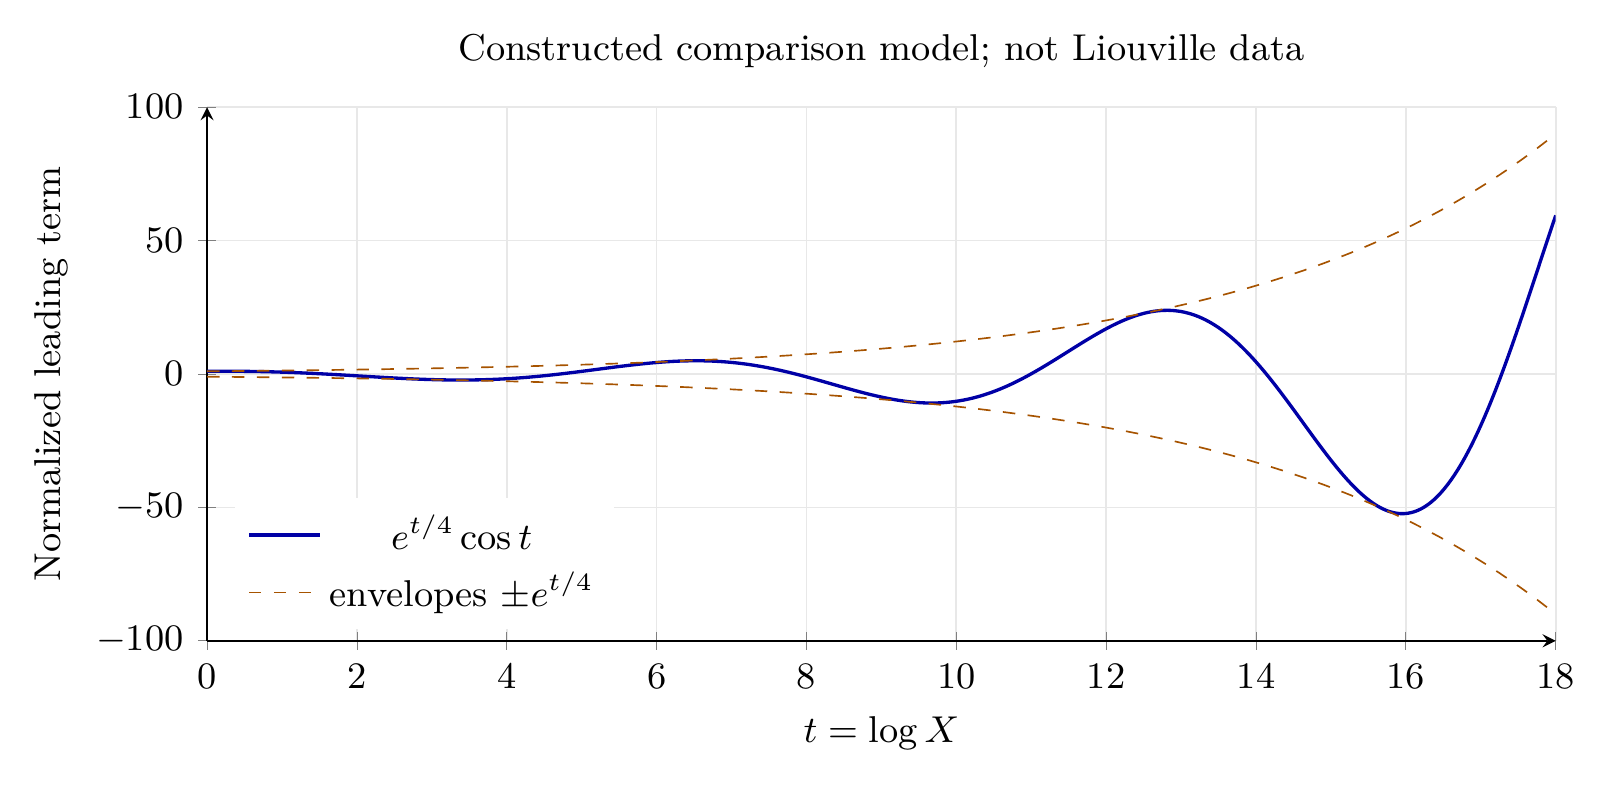
\includegraphics[width=\textwidth]{figures/model-abel-gap.png}
\caption{The phase-aligned model leading term, divided by
\(\varepsilon|\Gamma(3/4+i)|\sqrt X\), is
\(e^{t/4}\cos t\), where \(t=\log X\).
The dashed curves are its envelopes.
This is an analytic comparison model, not Liouville data or
a numerical test of RH.}\label{fig:model-growth}
\end{figure}

Theorem~\ref{thm:abel-obstruction} does not rule out a proof
that uses the full arithmetic structure of \(\lambda\).
Its coefficients are not required to be multiplicative.
It rules out a generic inference from bounded coefficients
and finitely many exact logarithmic moment cancellations to
the desired exponential-sum bound.
\footnote{The coefficients depend on \(k\), and the factor
\(\varepsilon\) need not have a positive lower bound as
\(k\to\infty\). The theorem constructs no single sequence
with every moment vanishing.}
The missing arithmetic estimate in
\eqref{eq:prime-tail-target} remains the point at which the
current RH argument stops. Adding the proved cancellations
at \(s=1\) does not fill that step.
